%\documentclass[draft, paper=a4, twoside=false, fontsize=12pt]{scrbook}
\documentclass[paper=a4, twoside=false, fontsize=12pt]{scrbook}

% General packages
\usepackage{sourdough}
\usepackage[
  paperwidth=210mm,
  paperheight=260mm,
  top=10mm,
  bottom=80mm,
  inner=10mm,
  outer=10mm,
  marginparsep=7mm,
  marginparwidth=48mm,
]{geometry}
\usepackage{showframe}
\usepackage{subcaption}

\pagenumbering{gobble}
% Basic attributes
\author{Hendrik Kleinwächter}
\title{The Sourdough Framework\\\texttt{tl;dr Version}}
\begin{document}
\maketitle

\section*{Starter maintenance}
\begin{flowchart}[!htb]
\documentclass[tikz]{standalone}
\usepackage{tikz}
\usepackage{siunitx}
\DeclareSIUnit\degF{\text{°}F}

\begin{document}
\begin{tikzpicture}[node distance = 3cm, auto]
  \node [block] (init) {\footnotesize Make a starter};
  \node [block, right of=init, node distance=3cm] (feed) {\footnotesize Feed your starter};
  \path [line] (init) -- (feed);
  \node [block, right of=feed, node distance=3cm] (wait_12_after_feed) {\footnotesize Wait 12 hours};
  \path [line] (feed) -- (wait_12_after_feed);
  \node [block, right of=wait_12_after_feed, node distance=3cm] (ready_question) {\footnotesize Perform readiness check};
  \path [line] (wait_12_after_feed) -- (ready_question);
  \node [block, below of=feed, node distance=3cm] (wait_12) {\footnotesize Wait 12 hours};
  \path [line] (wait_12) -- (feed);
  \node [decision, right of=ready_question, node distance=3.5cm] (is_bubbly) {\footnotesize Bubbly? Size Increase?};
  \path [line] (ready_question) -- (is_bubbly);
  \path [line] (is_bubbly) -- node{no} (wait_12);
  \node [decision, below of=is_bubbly, node distance=4.0cm] (check_smell) {\footnotesize Vinegary, or yogurt smell?};
  \path [line] (is_bubbly) -- node{yes} (check_smell);
  \node [block, below of=init, node distance=6cm] (make_dough) {\footnotesize Make your dough};
  \path [line] (check_smell) -- node{yes} (make_dough);
  \path [line] (check_smell) -- node{no} (wait_12);
\end{tikzpicture}
\end{document}

\caption*{Preparing your starter for baking}
\end{flowchart}

\begin{flowchart}[!htb]
\documentclass[tikz]{standalone}
\usepackage{tikz}
\usepackage{siunitx}
\DeclareSIUnit\degF{\text{°}F}

\begin{document}
\begin{tikzpicture}[node distance = 3cm, auto]
  \node [block] (init) {\footnotesize Make your bread dough};
  \node [decision, below of=init, node distance=3.5cm] (all_starter_used) {\footnotesize All starter used?};
  \path [line] (init) -- (all_starter_used);
  \node [block, right of=init, node distance=3cm] (use_dough) {\footnotesize Take 10g of your bread dough};
  \node [block, right of=all_starter_used, node distance=3cm] (use_starter) {\footnotesize Take all but not more than 10g of your starter};
  \path [line] (all_starter_used) -- node{yes} (use_dough);
  \path [line] (all_starter_used) -- node{no} (use_starter);
  \node [block, right of=use_dough, node distance=3cm] (feed_starter) {\footnotesize Feed using 1:5:5 ratio};
  \path [line] (use_dough) -- (feed_starter);
  \path [line] (use_starter) -- (feed_starter);
  \node [decision, right of=feed_starter, node distance=3cm] (bake_next_day_check) {\footnotesize Bake next day?};
  \path [line] (feed_starter) -- (bake_next_day_check);
  \node [block, right of=bake_next_day_check, node distance=3.5cm] (make_bread_dough) {\footnotesize Make bread dough again after 8-12 hours};
  \path [line] (bake_next_day_check) -- node{yes} (make_bread_dough);
  \node [decision, right of=use_starter, node distance=3cm] (bake_next_week_check) {\footnotesize Baking in next 2 weeks?};
  \node [block, right of=bake_next_week_check, node distance=3.5cm] (store_fridge) {\footnotesize Store starter in fridge at 4°C(40°F)};
  \path [line] (bake_next_week_check) -- node{yes} (store_fridge);
  \node [block, right of=store_fridge, node distance=3cm] (feed_after_fridge) {\footnotesize Feed again using 1:5:5 ration 8-12 hours before making dough};
  \path [line] (store_fridge) -- (feed_after_fridge);
  \path [line] (bake_next_day_check) -- node{no} (bake_next_week_check);
  \node [decision, below of=use_starter, node distance=3cm] (freezer_check) {\footnotesize Have a freezer?};
  \path [line] (bake_next_week_check) -- (store_fridge);
  \path [line] (bake_next_week_check) -- node{no} (freezer_check);
  \node [block, right of=freezer_check, node distance=3cm] (dry_starter) {\footnotesize Dry your starter};
  \node [block, below of=dry_starter, node distance=3cm] (freeze_starter) {\footnotesize Freeze your starter};
  \path [line] (freezer_check) -- node{no} (dry_starter);
  \path [line] (freezer_check) -- node{yes} (freeze_starter);
  \node [block, right of=dry_starter, node distance=3.5cm] (reactivate_freezer) {\footnotesize Reactivate starter for 3 days with daily 1:5:5 feedings};
  \path [line] (dry_starter) -- (reactivate_freezer);
  \path [line] (freeze_starter) -- (reactivate_freezer);
\end{tikzpicture}
\end{document}

\caption*{Maintaining your starter, change ratio as per starter hydration type}
\end{flowchart}

\clearpage{}
\section*{Baker math}
\begin{table}[!htb]
  \begin{tabular}{@{}r@{g }lrr@{ = }r@{}}
\toprule
\multicolumn{2}{c}{\thead{Ingredient}}& \thead{Percentage} & \multicolumn{2}{c}{\thead{Calculation}} \\ \midrule
1000& flour             &100\%        & 1000g of 1000g & 100\% \\ 
 600& water             & 60\%        & 600g of 1000g  &  60\% \\ 
 100& sourdough starter & 10\%        & 100g of 1000g  &  10\% \\ 
  20& salt              &  2\%         & 20g of 1000g  &   2\% \\ \bottomrule
\end{tabular}

  \caption*{An example table demonstrating how to properly calculate using
  baker's math}
\end{table}

\section*{Dough \& proofing}
\subsection*{Flat bread}
\subsubsection*{Ingredients}
\begin{tabular}{r@{}rl@{}}
\qty{400}{\gram} &~(\qty{100}{\percent}) & Flour (wheat, rye, corn, whatever
                                            you have at hand)\\
\qty{320}{\gram} &  (\qty{80}{\percent}) & Water, preferably at room
                                            temperature\\
\qty{80}{\gram}  &  (\qty{20}{\percent}) & Active sourdough starter\\
\qty{8}{\gram}   &   (\qty{2}{\percent}) & Salt\\
\end{tabular}

\subsubsection*{Instructions}
\begin{description}
\item[Prepare the dough] In a large mixing bowl, combine the flour and water.
    Mix until you have a shaggy dough with no dry spots.

    Add the sourdough starter and salt to the mixture. Incorporate them
    thoroughly until you achieve a smooth and homogenized dough.

\item[Fermentation:] Cover the bowl with a lid or plastic wrap. Allow the dough
    to rest and ferment until it has increased by at least \qty{50}{\percent}
    in size.  Depending on the temperature and activity of your starter, this
    can take anywhere from 4 to 24~hours.

\item[Cooking preparation:] Once the dough has risen, heat a pan over medium
    heat.  Lightly oil the pan, ensuring to wipe away any excess oil with a
    paper towel.

\item[Shaping and cooking:] With a ladle or your hands, scoop out a portion of
    the dough and place it onto the hot pan, spreading it gently like a
    pancake.

    Cover the pan with a lid. This traps the steam and ensures even cooking
    from the top, allowing for easier flipping later.

    After about 5~minutes, or when the bottom of the flatbread has a
    golden-brown crust, carefully flip it using a spatula.

    \emph{Adjusting cook time.} If the flatbread appears too dark, remember to
    reduce the cooking time slightly for the next one.  Conversely, if it's
    too pale, allow it to cook a bit longer before flipping.

    Cook the flipped side for an additional 5~minutes or until it's also
    golden brown.

\item[Storing:] Once cooked, remove the flatbread from the pan and place it on
    a kitchen towel. Wrapping the breads in the towel will help retain their
    softness and prevent them from becoming overly crisp.  Repeat the cooking
    process for the remaining dough.

\item[Serving suggestion:] Enjoy your sourdough flatbreads warm, paired with
    your favorite dips, spreads, or as a side to any meal.

\end{description}

\clearpage{}

\subsection*{Freestanding bread}
\begin{table}[!htb]
\begin{tabular}{@{}lrrrcr@{}}
\toprule
\thead{Ingredient}&                   & \thead{Percentage}  & \thead{Calculation}                                  \\ \midrule
Flour             & \qty{400}{g}      &  & \phantom{\qty{1000}{g} of \qty{1000}{g} \qty{100}{\percent}} \\ 
Whole-wheat flour & \qty{100}{g}      &  & \phantom{\qty{1000}{g} of \qty{1000}{g} \qty{100}{\percent}} \\ 
Total flour       &                   &\qty{100}{\percent}  & \qty{500}{g} \\
Water             &                   &\qty{60}{\percent} &\qty{300}{g}& \\
Sourdough starter &                   &\qty{10}{\percent} &\qty{50}{g}& \\
Salt              &                   &\qty{2}{\percent}  &\qty10{}{g}& \\ \midrule
Flour             & \phantom{\qty{1000}{g}} &\qty{100}{\percent}  & \phantom{\qty{1000}{g} of \qty{1000}{g} \qty{100}{\percent}} \\ 
Water             & & & \\
Sourdough starter & & & \\
Salt              & & & \\ \midrule
Flour             & \phantom{\qty{1000}{g}} &\qty{100}{\percent}  & \phantom{\qty{1000}{g} of \qty{1000}{g} \qty{100}{\percent}} \\ 
                  & & & \\
                  & & & \\
                  & & & \\
                  & & & \\ \bottomrule
\end{tabular}
  \caption*{Table for your own calculation using baker's math}
\end{table}
\begin{flowchart}[!htb]
\begin{tikzpicture}[node distance = 3.2cm, auto]
  \node [start] (init) {Ready starter};
  \node [block, right of=init] (mix_ingredients) {Mix ingredients};
  \node [block, right of=mix_ingredients] (dough_strength) {Create dough strength};
  \node [block, right of=dough_strength] (bulk) {Bulk ferment};
  \node [decision, below of=bulk] (divide_test) {Making one loaf?};
  \node [block, right of=divide_test] (divide) {Divide};
  \node [block, below of=divide] (preshape) {Preshape};
  \node [block, below of=divide_test] (shape) {Shape};
  \node [block, left of=shape] (proof) {Proof};
  \node [success, left of=proof] (bake) {Bake};
  \path [line] (init) -- (mix_ingredients);
  \path [line] (mix_ingredients) -- (dough_strength);
  \path [line] (dough_strength) -- (bulk);
  \path [line] (bulk) -- (divide_test);
  \path [line] (divide_test) -- node{yes} (shape);
  \path [line] (divide_test) -- node{no} (divide);
  \path [line] (divide) -- (preshape);
  \path [line] (preshape) -- (shape);
  \path [line] (shape) -- (proof);
  \path [line] (proof) -- (bake);
\end{tikzpicture}


\end{flowchart}
\begin{flowchart}[!htb]
\begin{tikzpicture}[node distance = 3cm, auto]
  \node [start] (init) {\footnotesize Homogenize recipe ingredients};
  \node [block, right of=init, node distance=3cm] (wait1) {\footnotesize Wait 15~minutes};
  \path [line] (init) -- (wait1);
  \node [block, right of=wait1, node distance=3cm] (knead1) {\footnotesize Knead 5~minutes};
  \path [line] (wait1) -- (knead1);
  \node [block, right of=knead1, node distance=3cm] (wait2) {\footnotesize Wait 15~minutes};
  \path [line] (knead1) -- (wait2);
  \node [decision, below of=wait2, node distance=3cm] (windowpane_test) {\footnotesize Window-pane?};
  \path [line] (wait2) -- (windowpane_test);
  \path [line] (windowpane_test) -- node{no} (knead1);
  \node [decision, left of=windowpane_test, node distance=4.5cm] (more_water) {\footnotesize Bassinage for more water?};
  \path [line] (windowpane_test) -- node{yes} (more_water);
  \node [block, left of=more_water, node distance=4.5cm] (add_water) {\footnotesize Add water};
  \path [line] (more_water) -- node{yes} (add_water);
  \path [line] (add_water) -- (knead1);
  \node [block, below of=add_water, node distance=4cm] (wait3) {\footnotesize Wait 15~minutes};
  \path [line] (add_water) -- (wait3);
  \node [decision, right of=wait3, node distance=4.5cm] (dough_sample) {\footnotesize Aliquot sample?};
  \path [line] (wait3) -- (dough_sample);
  \path [line] (more_water) -- node{no} (dough_sample);
  \node [block, right of=dough_sample, node distance=4.5cm] (dough_ball) {\footnotesize Make round dough ball};
  \path [line] (dough_sample) -- node{no} (dough_ball);
  \node [block, below of=dough_sample, node distance=3cm] (extract_sample) {\footnotesize Extract sample};
  \path [line] (dough_sample) -- node{yes} (extract_sample);
  \path [line] (extract_sample) -- (dough_ball);
  \node [success, below of=dough_ball, node distance=3cm] (begin_bulk) {\footnotesize Begin bulk fermentation};
  \path [line] (dough_ball) -- (begin_bulk);
\end{tikzpicture}

\end{flowchart}

\begin{flowchart}[!htb]
\begin{tikzpicture}[node distance = 3cm, auto]
  \node [start] (init) {Bulk fermentation};
  \node [block, right of=init, node distance=4cm] (check_dough) {Check the dough};
  \node [block, right of=check_dough, node distance=4cm] (size_increase) {Check dough size increase};
  \node [block, below of=size_increase, node distance=2cm] (ph_value) {Check dough pH value};
  \node [block, below of=ph_value, node distance=2cm] (smell) {Check dough smell};
  \node [decision, right of=size_increase, node distance=4cm] (dough_ready) {Dough ready?};
  \node [success] at(dough_ready |- smell) (divide_preshape) {Divide and preshape};
  \node [decision, above of=size_increase] (dough_flattened) {Dough flattened out?};
  \node [block, above of=check_dough] (wait_60_minutes) {Wait\\ 60~minutes};
  \node [block, above of=wait_60_minutes] (stretch_fold) {Stretch and fold};

  \path [line] (init) -- (check_dough);
  \path [line] (check_dough) -- (size_increase);
  % Tricks not to get double lines
  \path [line] (check_dough) ++(2, -2) -- node{or} (ph_value);
  \path [line] (check_dough) ++(2, 0) -- node{} ++(0, -4) -- node{or} (smell);
  \path [line] (check_dough) ++(2, -4) -- node{or} (smell);
  \path [line] (size_increase) -- (dough_ready);
  % Same tricks not to get double lines and also we do _not_ want arrows
  \path [draw, thick] (ph_value) -- node{} ++(2, 0);
  \path [draw, thick] (smell) -| node{} ++(2, 4);
  \path [line] (dough_ready) -- node{Yes} (divide_preshape);
  \path [line] (dough_ready) |- node[right=3pt]{no} (dough_flattened);
  \path [line] (dough_flattened) |- node[right=3pt]{yes} (stretch_fold);
  \path [line] (dough_flattened) -- node{No} (wait_60_minutes);
  \path [line] (stretch_fold) -- (wait_60_minutes);
  \path [line] (wait_60_minutes) -- (check_dough);
\end{tikzpicture}

\end{flowchart}
\begin{figure*}[!htb]
  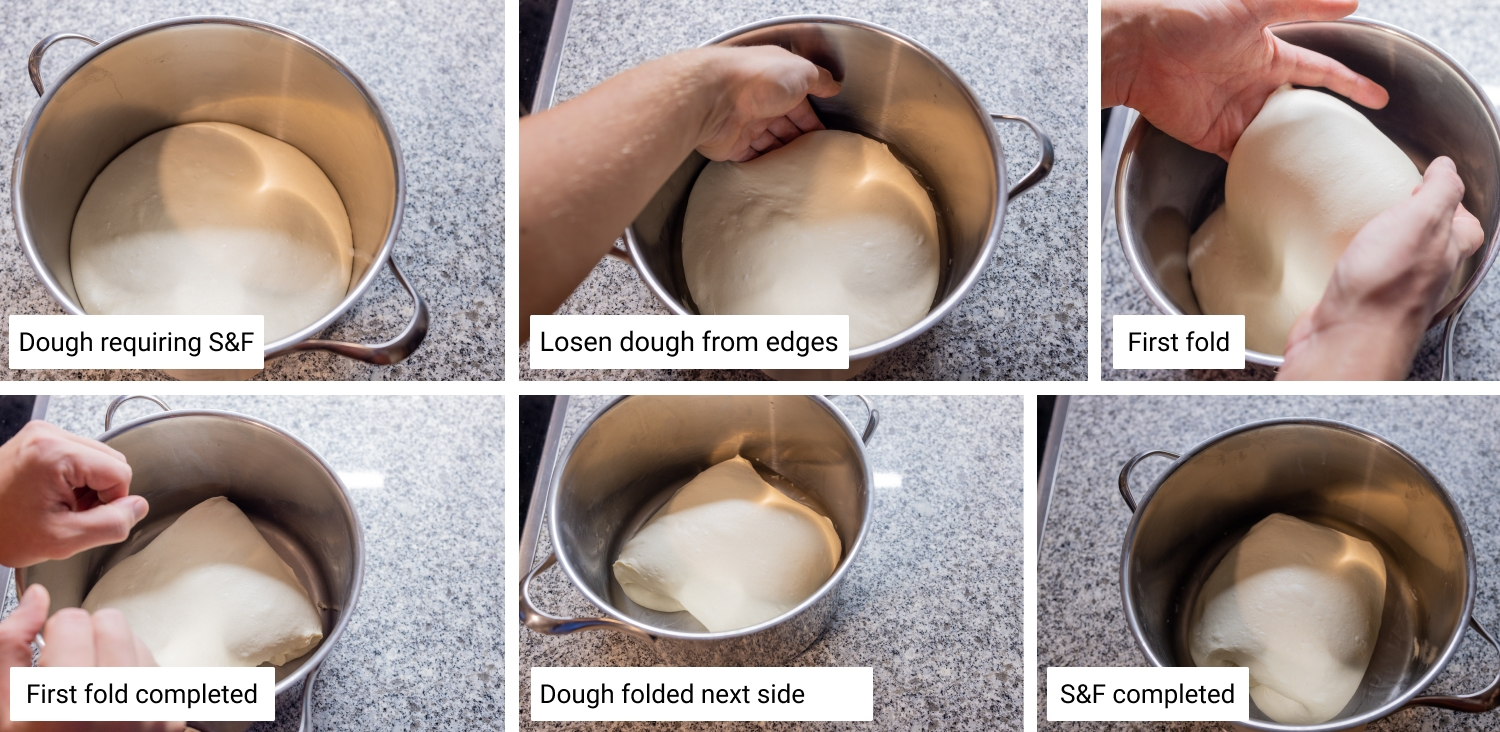
\includegraphics[width=\textwidth]{stretch-and-fold-steps}
  \caption*{An overview of the steps involved to perform stretch and folds for
  wheat-based doughs.}%
\end{figure*}
\clearpage{}

\section*{Shaping}
\begin{flowchart}[!htb]
\begin{tikzpicture}[node distance = 3cm, auto]
  \node [decision] (init) {\footnotesize Room temperature proofing?};
  \node [decision, right of=init, node distance=9cm] (retard_bake_decision) {\footnotesize Bake in less than 10 hours from now?};
  \node [block, below of=init, node distance=4cm] (poke) {\footnotesize Poke the dough};
  \node [block, right of=poke, node distance=4cm] (wait_poke) {\footnotesize Wait 15 minutes};
  \node [decision, below of=poke, node distance=3cm] (dent_visible_decision) {\footnotesize Dent still visible after 1 minute?};
  \node [block, right of=dent_visible_decision, node distance=4cm] (bake) {\footnotesize Score and bake};
  \node [block, below of=retard_bake_decision, node distance=3cm] (wait_retard) {\footnotesize Wait 15 minutes};
  \node [block, below of=wait_retard, node distance=3cm] (retard) {\footnotesize Proof in fridge at 4°C (40°F)};
  \node [block, right of=wait_retard, node distance=3cm] (move_to_fridge) {\footnotesize Move dough directly to fridge};
  \path [line] (init) -- node{yes} (poke);
  \path [line] (init) -- node{no} (retard_bake_decision);
  \path [line] (poke) -- (dent_visible_decision);
  \path [line] (dent_visible_decision) -- node{yes} (bake);
  \path [line] (dent_visible_decision) -- node{no} (wait_poke);
  \path [line] (wait_poke) -- (poke);
  \path [line] (retard_bake_decision) -- node{yes} (wait_retard);
  \path [line] (retard_bake_decision) -- node{no} (move_to_fridge);
  \path [line] (wait_retard) -- (retard);
  \path [line] (move_to_fridge) -- (retard);
  \path [line] (retard) -- (bake);
\end{tikzpicture}

\end{flowchart}

\begin{figure*}[!htb]
\begin{subfigure}{.475\linewidth}
  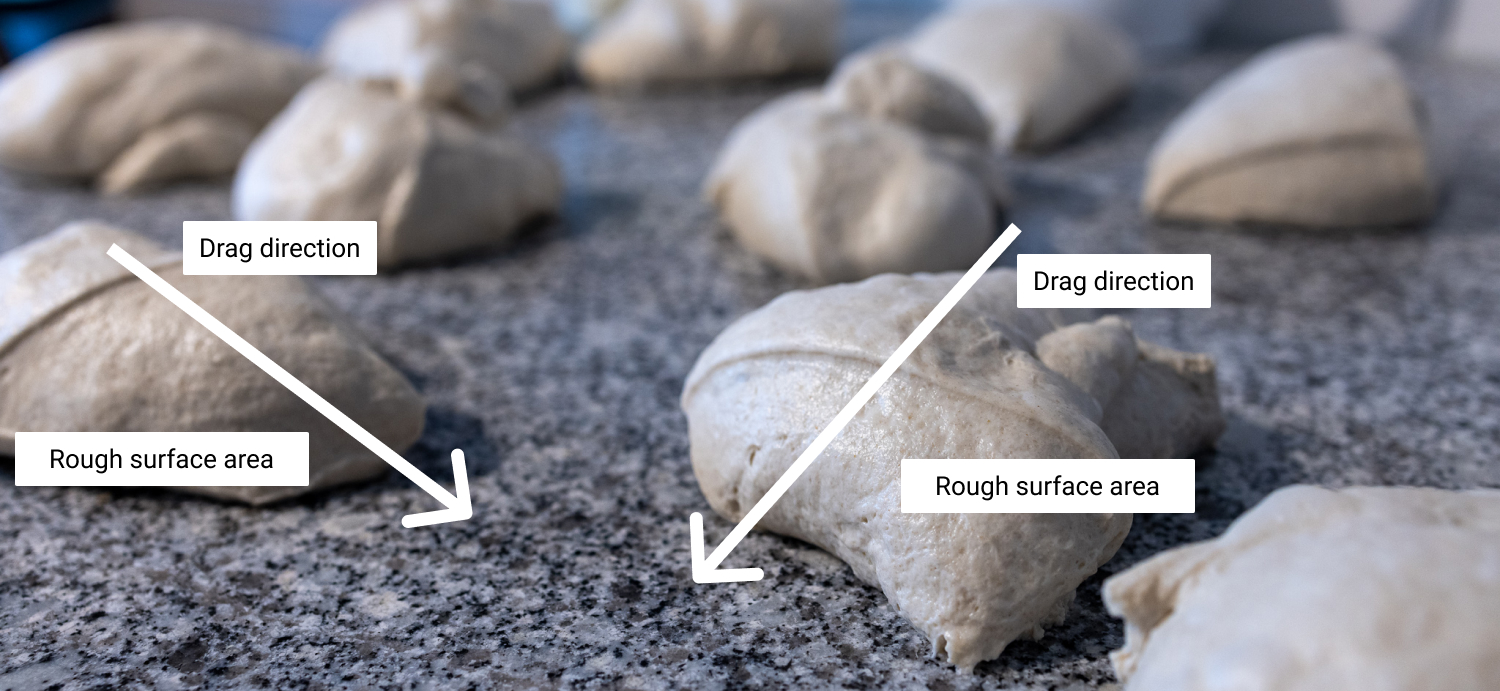
\includegraphics[width=\linewidth]{preshape-direction}
  \caption*{Preshaping: Drag the dough in the direction of the rough surface
  area.}%
\end{subfigure}
\begin{subfigure}{.475\linewidth}
  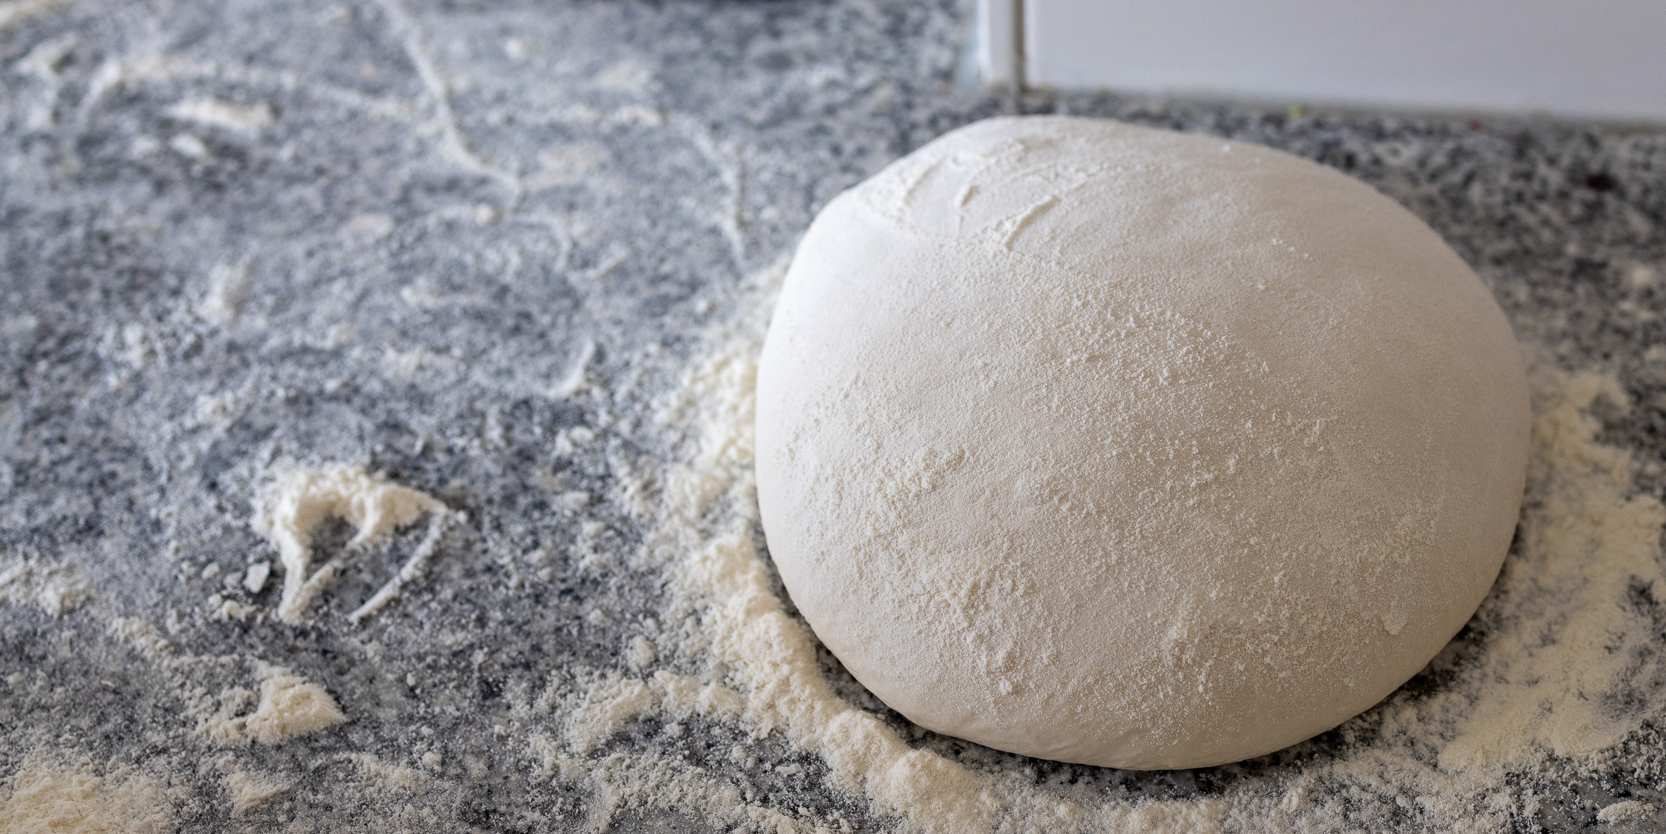
\includegraphics[width=\linewidth]{step-1-flour-applied}
  \caption*{Step 1: Apply flpour to the dough's surface.}%
\end{subfigure}\hfill % <-- "\hfill"
\medskip % create some *vertical* separation between the graphs
\begin{subfigure}{.475\linewidth}
  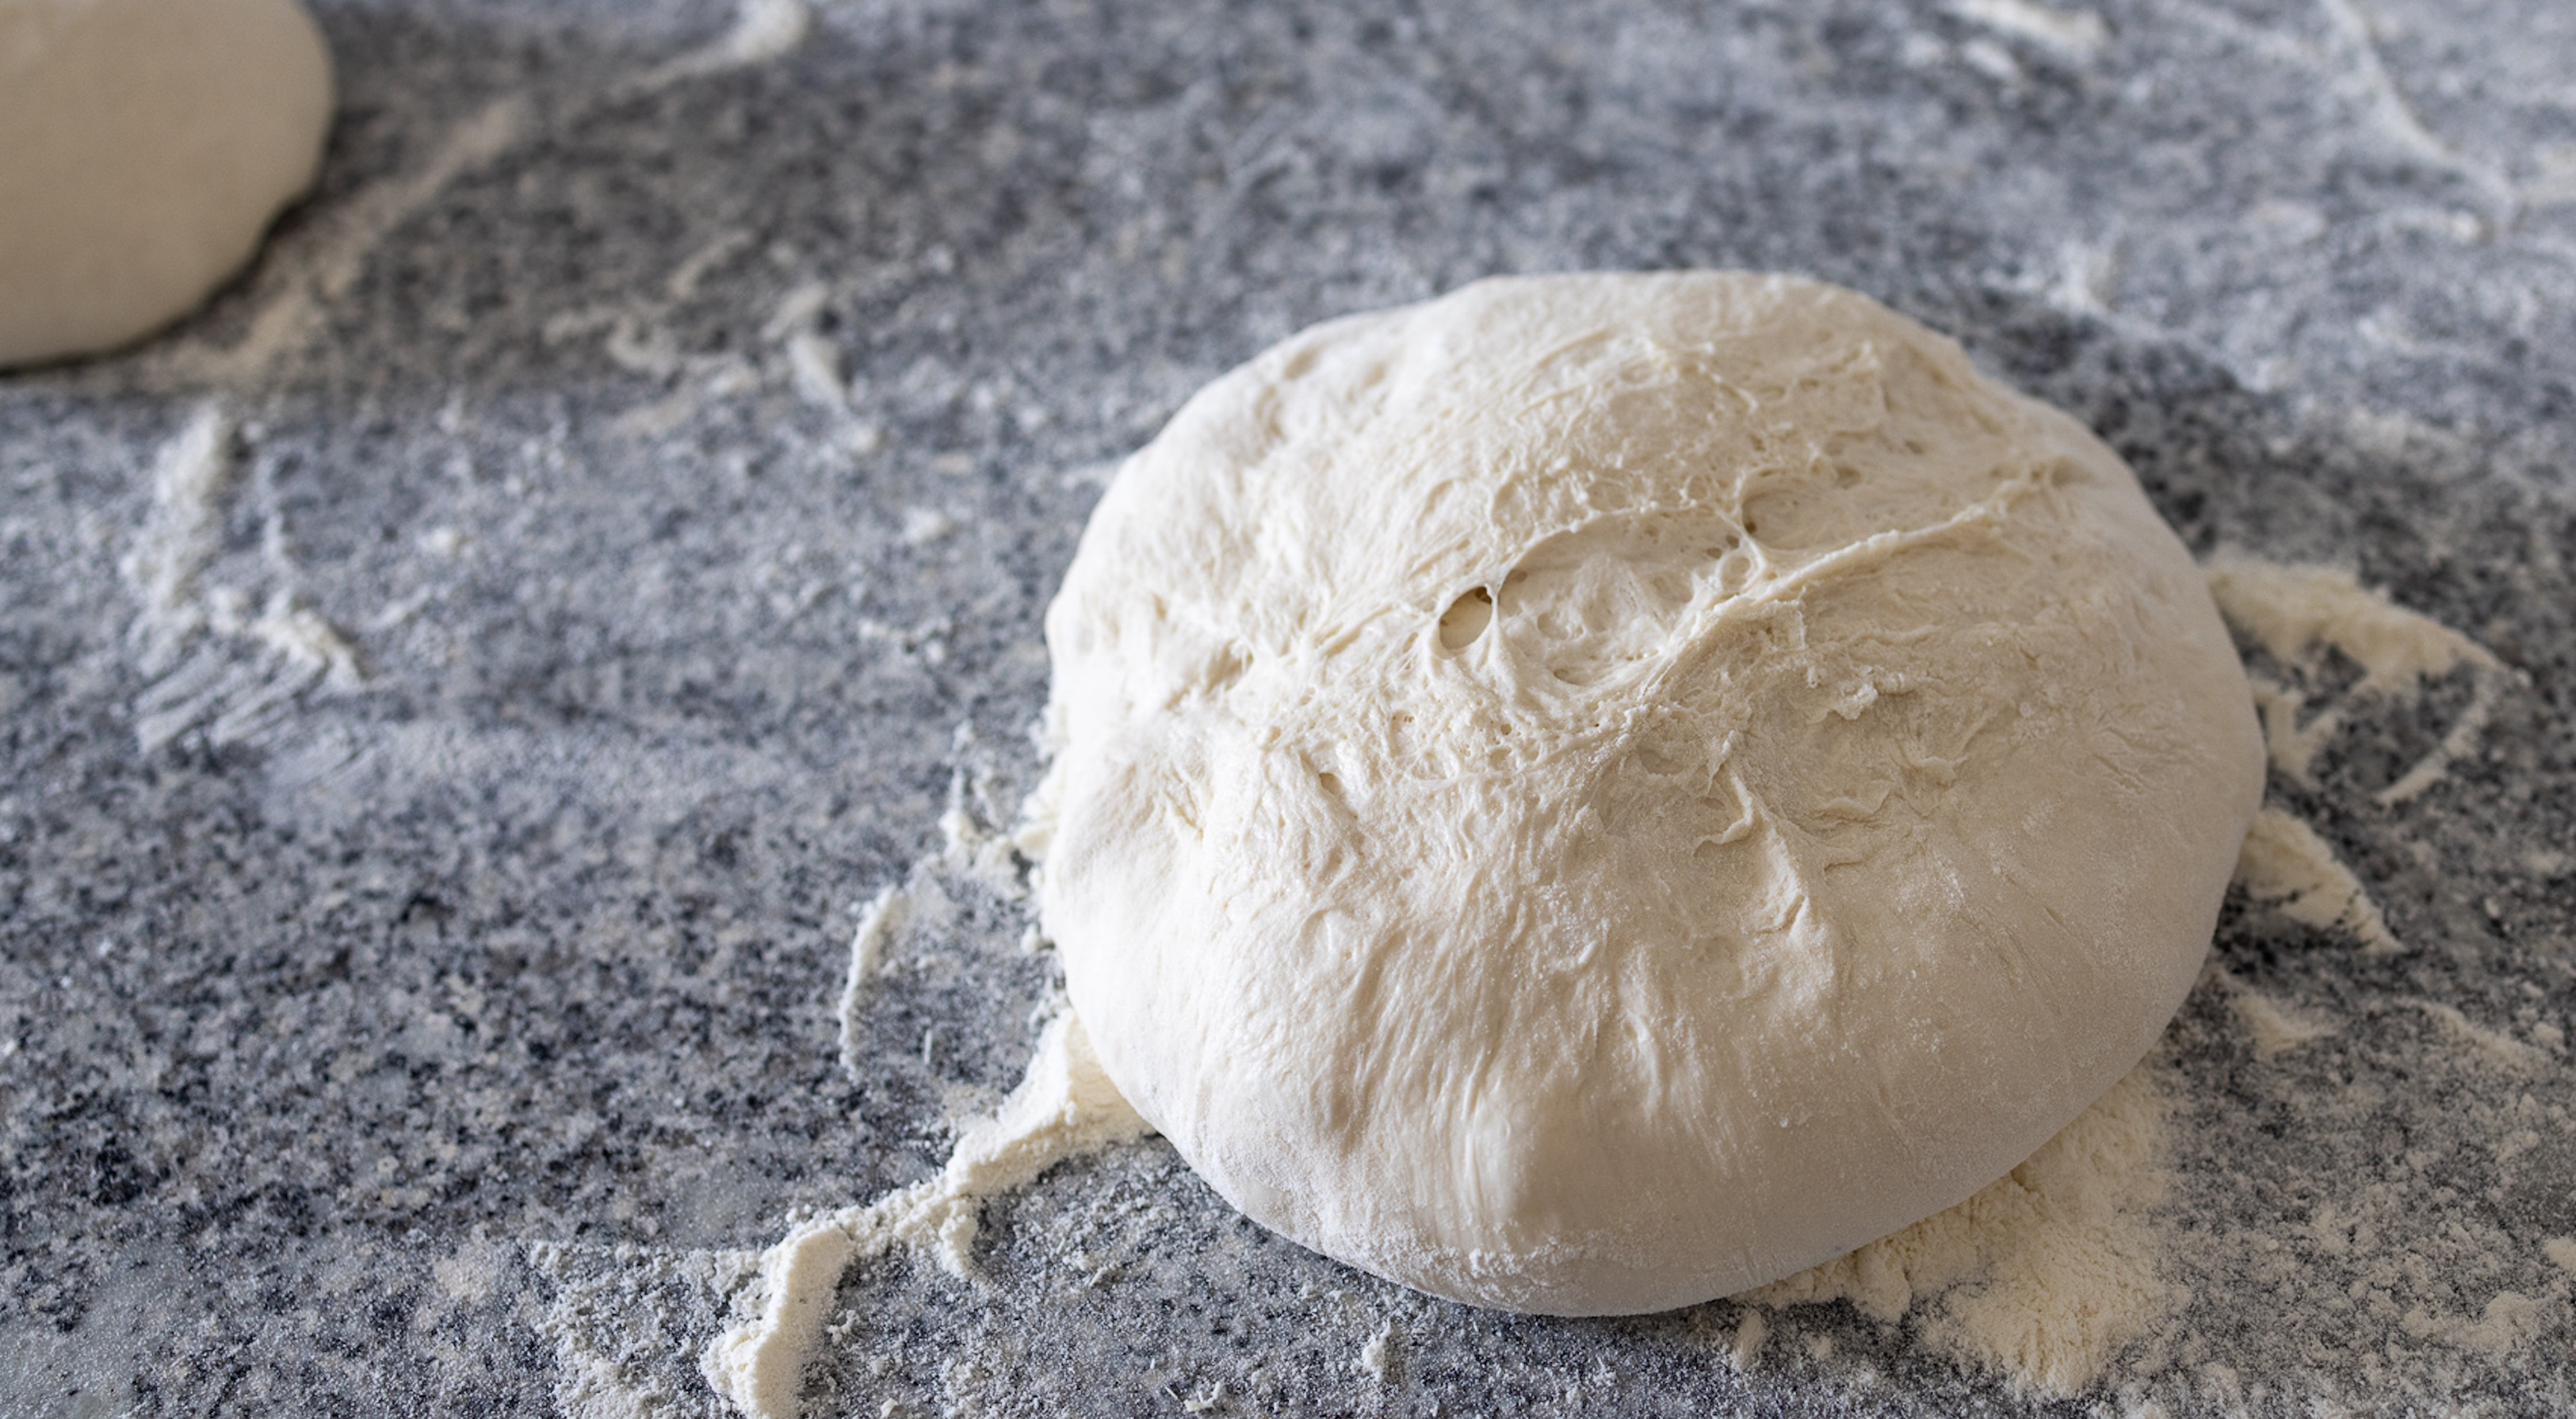
\includegraphics[width=\linewidth]{step-2-flipped-over}
  \caption*{Step 2: Flipp-over dough. Note how the sticky side is facing you
  while the floured side is facing the countertop.}
\end{subfigure}\hfill % <-- "\hfill"
\begin{subfigure}{.475\linewidth}
  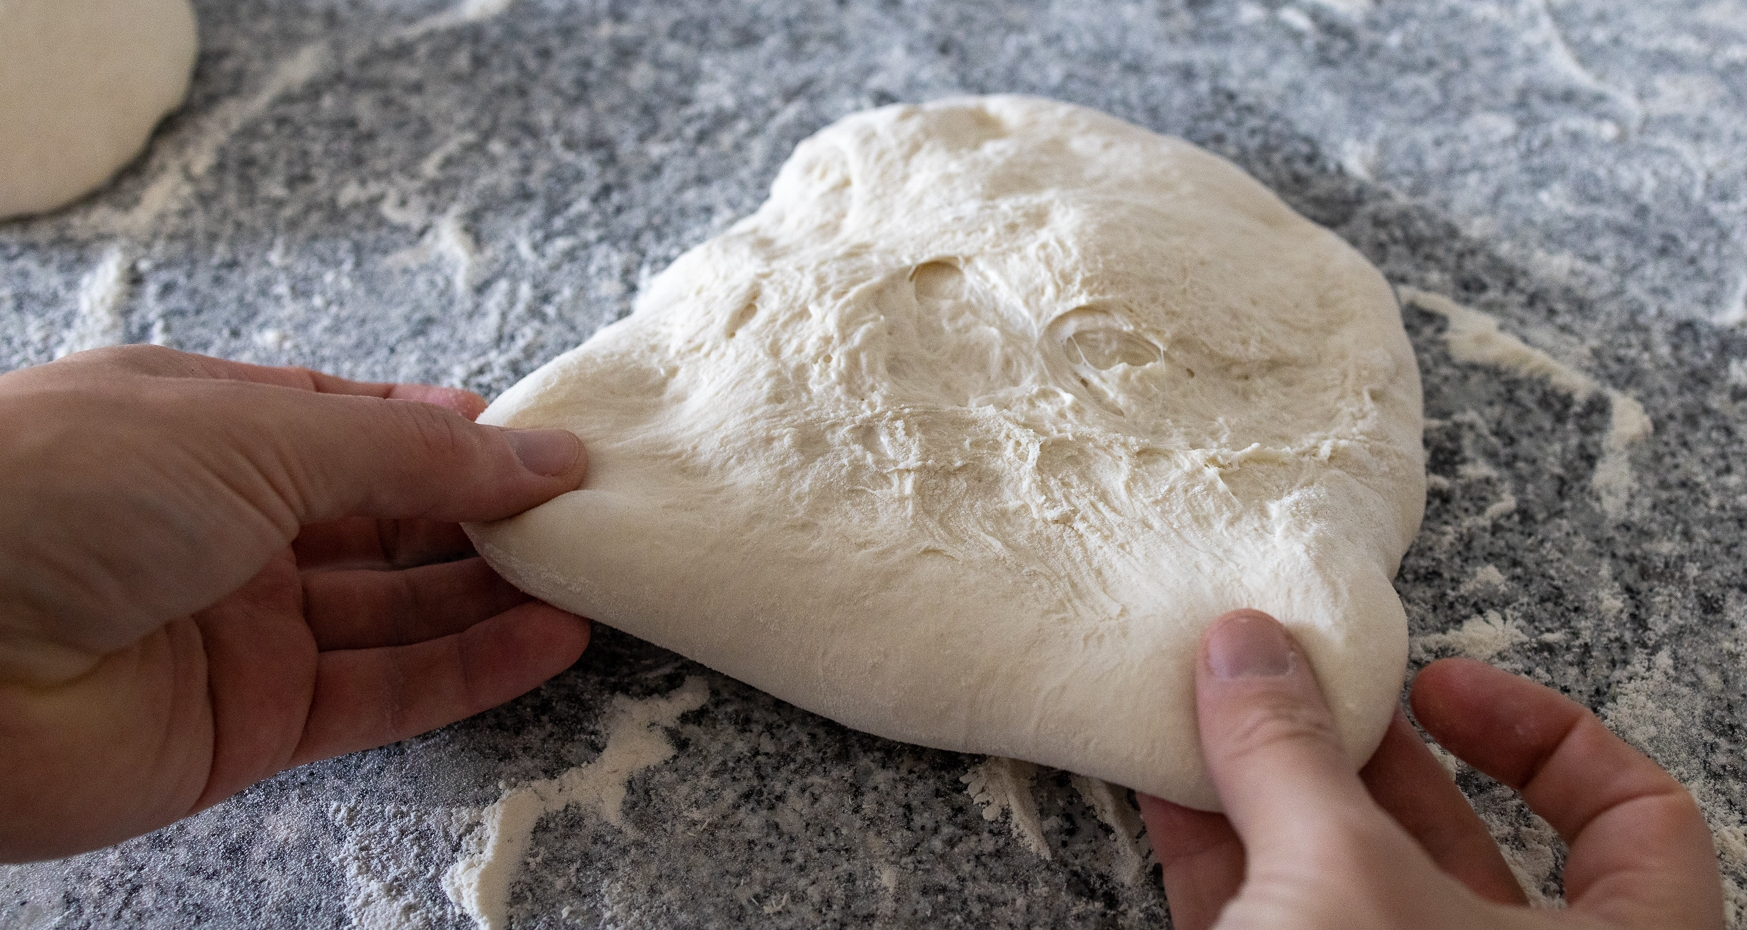
\includegraphics[width=\linewidth]{step-3-rectangular}
  \caption*{Step 3: Make the dough rectangular, keep the sticky side facing
  you while the floured side is facing the countertop.}%
\end{subfigure}
\caption*{First steps of shaping process}
\end{figure*}

\begin{figure*}[htb!]
  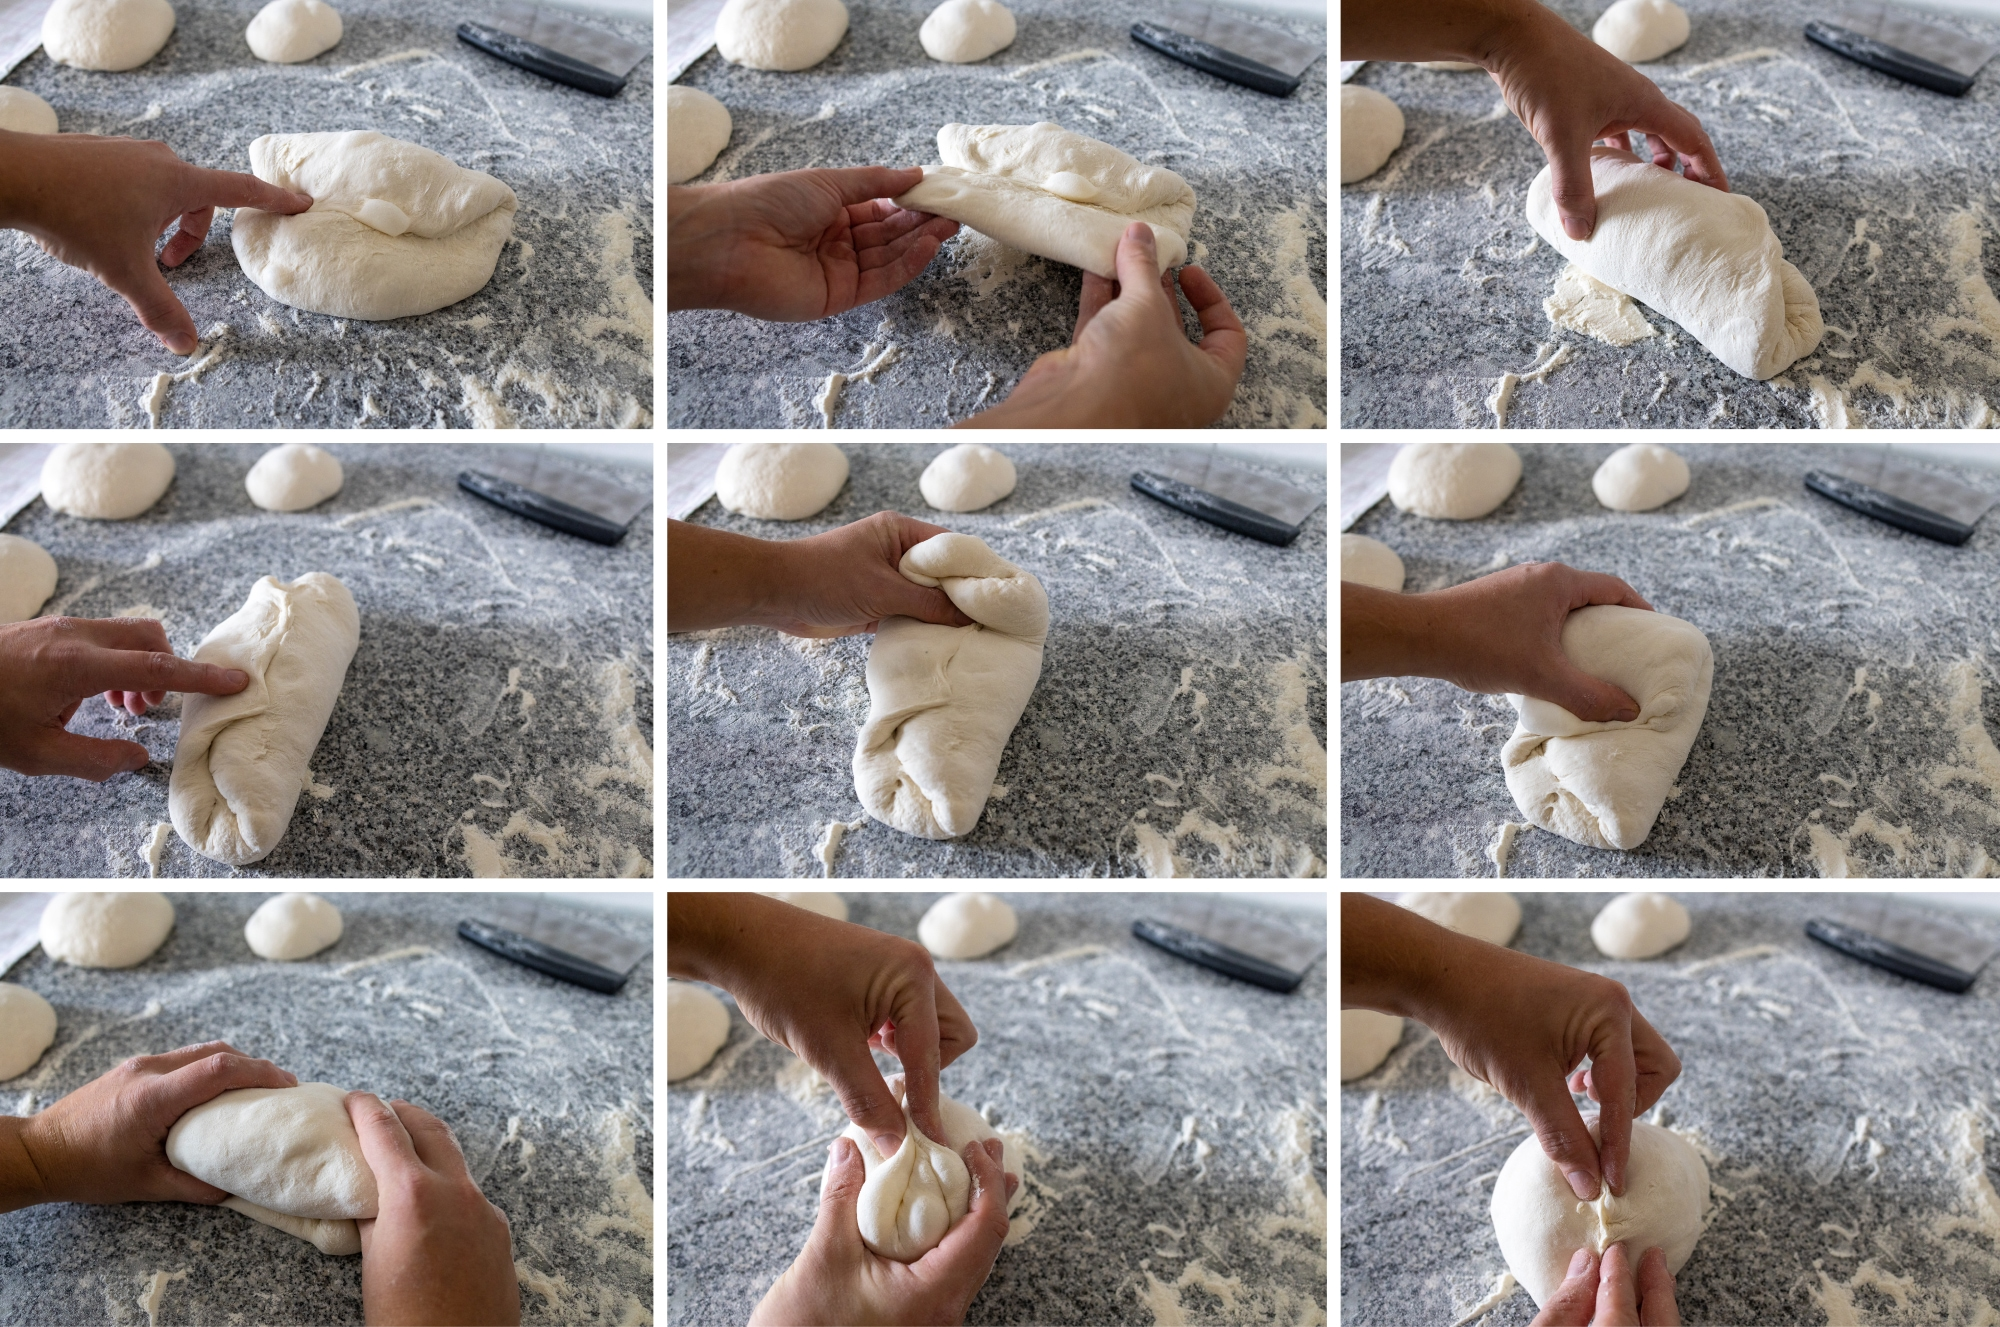
\includegraphics[width=\textwidth]{step-4-folding}
  \caption*{Step 4: The process of folding a batard.  Note how the rectangle
  is first glued together and then rolled inwards to create a dough roll.
  Utimately the edges are sealed to create a more uniform dough.}%
\end{figure*}
\clearpage{}

\section*{Baking}
\begin{flowchart}[!htb]
\begin{tikzpicture}[node distance = 3cm, auto]
  \node [block] (heat_oven) {\footnotesize Heat oven to 230°C (446°F) for 30 minutes};
  \node [block, right of=heat_oven, node distance=3cm] (score_dough) {\footnotesize Score your dough};
  \node [decision, right of=score_dough, node distance=4cm] (decide_steam) {\footnotesize Choose your steaming method};
  \node [block, below of=heat_oven, node distance=4cm] (inverted_tray_method) {\footnotesize Inverted tray method};
  \node [block, right of=inverted_tray_method, node distance=3cm] (dutch_oven) {\footnotesize Dutch oven};
  \node [block, right of=dutch_oven, node distance=3cm] (steam_injection) {\footnotesize Steam injection oven};
  \node [block, below of=inverted_tray_method, node distance=3cm] (bake_30) {\footnotesize Bake dough for 30 minutes with steam};
  \node [block, right of=bake_30, node distance=3cm] (remove_steam) {\footnotesize Remove source of steam};
  \node [block, right of=remove_steam, node distance=3cm] (build_crust) {\footnotesize Build the crust};
  \node [block, right of=build_crust, node distance=3cm] (finish_baking) {\footnotesize Stop baking 10--30 minutes later depending on crust preference};
  \path [line] (heat_oven) -- (score_dough);
  \path [line] (score_dough) -- (decide_steam);
  \path [line] (decide_steam) -- (inverted_tray_method);
  \path [line] (decide_steam) -- (dutch_oven);
  \path [line] (decide_steam) -- (steam_injection);
  \path [line] (steam_injection) -- (bake_30);
  \path [line] (inverted_tray_method) -- (bake_30);
  \path [line] (dutch_oven) -- (bake_30);
  \path [line] (bake_30) -- (remove_steam);
  \path [line] (remove_steam) -- (build_crust);
  \path [line] (build_crust) -- (finish_baking);
\end{tikzpicture}

\caption*{Summary of bread bakign process}
\end{flowchart}

\begin{flowchart*}[!htb]
\begin{tikzpicture}[node distance = 3cm, auto]
  \node [start] (heat_oven) {Preheat DO to \qty{230}{\degreeCelsius} (\qty{446}{\degF}) for 30~minutes};
  \node [block, right of=heat_oven] (remove_oven) {Remove DO from oven };
  \node [block, right of=remove_oven] (open_load_dough) {Open DO \& load your dough};
  \node [block, right of=open_load_dough] (score) {Score your dough};
  \node [block, right of=score] (spritz) {Spritz dough with water};
  \node [block, below of=spritz] (close) {Close DO};
  \node [block, left of=close] (back_oven) {Place DO back in oven};
  \node [block, left of=back_oven] (bake) {Bake 30~minutes at \qty{230}{\degreeCelsius} (\qty{446}{\degF})};
  \node [decision, below right= 5cm and -1 cm of heat_oven]  (is_ready_check)
        {Core temperature \qty{92}{\degreeCelsius} (\qty{197}{\degF})?};
  \node [block, below of=is_ready_check, node distance=4cm] (wait_5_minutes) {Wait\\ 5 minutes};
  \node [block, right of=is_ready_check, node distance=4cm] (remove_do_lid) {Remove DO lid};
  \node [decision, right of=remove_do_lid, node distance=3.5cm] (dark_enough_decision) {Crust color dark enough?};
  \node [success, below of=dark_enough_decision, node distance=4cm] (finish_baking) {Bread is finished};
  \node [block, right of=dark_enough_decision, node distance=3.5cm] (bake_5_more_minutes) {Bake another 5~minutes};
  \path [line] (heat_oven) -- (remove_oven);
  \path [line] (remove_oven) -- (open_load_dough);
  \path [line] (open_load_dough) -- (score);
  \path [line] (score) -- (spritz);
  \path [line] (spritz) -- (close);
  \path [line] (close) -- (back_oven);
  \path [line] (back_oven) -- (bake);
  \path [line] (bake.west) -- node{} ++(-2, 0) -| (is_ready_check.north);
  \path [line] (is_ready_check) -- node{yes} (remove_do_lid);
  \path [line] (is_ready_check) -- node{no} (wait_5_minutes);
  \path [line] (wait_5_minutes.west) -- node{} ++(-1.5, 0) |- (is_ready_check.west);
  \path [line] (remove_do_lid) -- (dark_enough_decision);
  \path [line] (dark_enough_decision) -- node{yes} (finish_baking);
  \path [line] (dark_enough_decision) -- node{no} (bake_5_more_minutes);
  \path [line] (bake_5_more_minutes.east) -- node{} ++(1, 0) -- node{} ++(0, 2.3) -| (dark_enough_decision.north);
\end{tikzpicture}

\caption*{Bakign with a Dutch Oven}
\end{flowchart*}

\begin{flowchart}[!htb]
\begin{tikzpicture}[node distance = 3cm, auto]
  \node [block] (init) {\footnotesize Place water tray and stone in oven};
  \node [block, right of=init] (heat_oven) {\footnotesize Heat oven to  \qty{230}{\degreeCelsius} (\qty{446}{\degF}) for 30~minutes};
  \node [block, right of=heat_oven] (score_your_dough) {\footnotesize Score your dough};
  \node [block, right of=score_your_dough] (spritz) {\footnotesize Spritz your dough with water};
  \node [block, right of=spritz] (load_tray) {\footnotesize Place non-preheated inverted tray in oven};
  \node [block, below of=load_tray, node distance=4cm] (load_doughs) {\footnotesize Load doughs into oven};
  \node [block, left of=load_doughs, node distance=3cm] (load_water) {\footnotesize Place water in heated water tray};
  \node [block, left of=load_water, node distance=3cm] (bake) {\footnotesize Bake 30~minutes or until core temperature is  \qty{92}{\degreeCelsius} (\qty{197}{\degF})};
  \node [block, left of=bake, node distance=3cm] (remove_steam) {\footnotesize Remove steam source and top tray};
  \node [block, left of=remove_steam, node distance=3cm] (finish) {\footnotesize Bake at least another 10~minutes or until crust has your desired color};
  \path [line] (init) -- (heat_oven);
  \path [line] (heat_oven) -- (score_your_dough);
  \path [line] (score_your_dough) -- (spritz);
  \path [line] (spritz) -- (load_tray);
  \path [line] (load_tray) -- (load_doughs);
  \path [line] (load_doughs) -- (load_water);
  \path [line] (load_water) -- (bake);
  \path [line] (bake) -- (remove_steam);
  \path [line] (remove_steam) -- (finish);
\end{tikzpicture}

\caption*{Bakign with the inverted tray method}
\end{flowchart}
\clearpage{}
\end{document}
